\makeatletter
\let\my@xfloat\@xfloat
\makeatother
\documentclass[compressed,final,notitlepage,narroweqnarray,inline,twoside,]{ieee}

\makeatletter
\def\@xfloat#1[#2]{
\my@xfloat#1[#2]
\def\baselinestretch{1}
\@normalsize \normalsize
}
\makeatother
\usepackage{makeidx}
\usepackage{tikz} 
\usepackage{graphicx}
\usepackage{caption}
\usepackage{subcaption}
\usepackage[caption=false]{subfig}
\usepackage{amsmath} 
\usepackage{amsfonts}
\usepackage{float}
\restylefloat{figure}
\usepackage[boxed]{algorithm2e}
\setlength{\parindent}{0cm}

\usepackage{framed}

\title[TITLE]{Implementation and Analysis of Monte-Carlo Tree Search.}
\author{By,Tamis van der Laan \& Author Samuel Austin }

\begin{document}
\maketitle

\begin{abstract}
We implemented a Monte Carlo Tree Search algorithm as part of an AI for playing various zero sum, perfect information, deterministic, discrete and sequential games. An analysis was performed on the performance of the algorithm and the benefit of randomization in the algorithm.
\end{abstract}

\section{Introduction}
Finding a solution to many combinatorial problems requires searching through a large tree to find an answer. This is often encountered in artificial intelligence where a large sequence of choices need to be made to reach a certain outcome. An example of this is the playing of games such as chess, checkers and tic-tac-toe. What makes these problems harder is that there is an opponent whose actions can not be predicted.

Any algorithm trying to tackle this problem will not only have to find the best move at a certain state but also take into account the possible moves that the opponent can perform. Due to the exponentially large number of possibilities it is not feasible to analyze all combinations of actions. To find a good action to take, heuristics specific to the problem can be used to reduce the size of the search space. Also global and local search techniques can be used to sample the possibilities and make an estimation of which actions will lead to a positive outcome.

Algorithms which do random sampling of the search space have been shown to be quite successful. In particular, Monte Carlo Tree Search is a popular algorithm for estimating solutions to these problems. In this paper we implement the Monte Carlo Tree Search algorithm in order to analyze its performance and draw conclusions on the benefits of the randomized aspects of the algorithm.

\section{Algorithm Description}
Monte Carlo Tree Search is a popular algorithm used in the context of games to approximate the best move.\cite{MCTS} The algorithm is also used in other settings then games such as planning and optimization \& control problems. The basic component of the Monte Carlo Tree Search Algorithm relies on a more simple version called the Monte Carlo Search Algorithm. This algorithm approximates the chance of winning given a state and a move in the game by performing many random walks down the tree to the leaves. Every transition towards the leaves signifies a move in the game leading to a new node which represents a state in the game. By counting the score with respect to the player the best move can be selected.

\subsection{Data Structure}
As the name of the algorithm suggests, a tree structure is used to represent a certain state and the possible actions for reaching another state. Each node in the tree represents a state and an edge represents the action required to reach that state. Each node also has a score assigned to it, where the higher the score the higher the probability of a good outcome for the algorithm.

\subsection{Algorithm}
The Monte Carlo Tree Search Algorithm makes use of the tree data structure described above in the following manner. At the beginning of the game a single root node is created defining the tree which represents the current state of the game. Then this tree is dynamically expanded, namely a node from the tree is randomly selected based on weighted probabilities governed by the UCT equation (see tree policy section) which is called the tree policy. After selection has taken place a random move is uniformly selected and a new node is created which captures the state transition from the previous state towards the new state by executing the move in question. This step is called the expansion step. In case that the node for that new state already exists it is simply selected instead of created. The next step in the process is to use the basic Monte Carlo Search algorithm multiple times. This step is called the exploration step and it counts the number of wins compared to the number of trials of the Monte Carlo Searches. Once this exploration step has finished the results are propagated up the tree towards the root node in the back propagation step.
\begin{figure*}[ht]
        \centering
        \begin{subfigure}[b]{1\textwidth}
                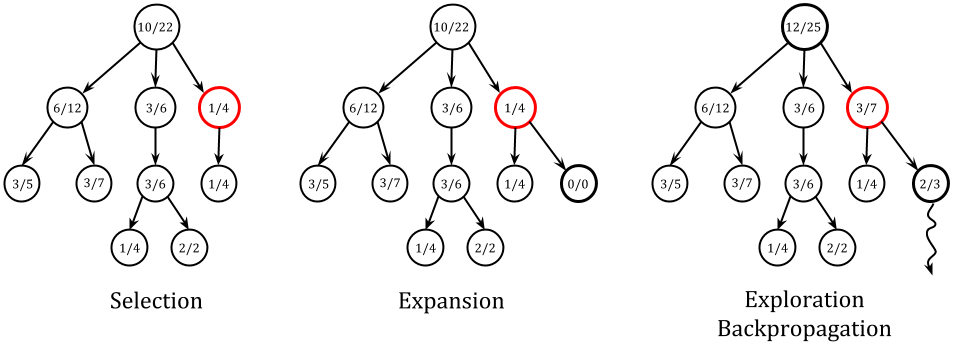
\includegraphics[width=\textwidth]{../images/mcts_algorithm}
        \end{subfigure}
        \vspace{-10pt}
        \caption{ This figure illustrates the selection, expansion, exploration and backpropagation process of the MCTS algorithm.}
        
        \label{fig:1}
\end{figure*}

\subsection{Tree Policy}
The tree policy guides the way in which the tree is being explored. It trades of widening the tree i.e. finding new interesting moves and deepening the tree i.e. exploring interesting moves further down. The policy is embodied in the form of a equation in our case we used one of the most popular policies the UCT policy:

$UCT = \bar{X}_j+2C_p \sqrt{\frac{2 ln(n)}{n_j}}, \mbox{ with } C_p = 1/\sqrt{2}$

This equation gives a score to each node in the tree. One of the nodes is then selected at random weighted with probability equal to the UTC score. The $\bar{X}_j$ term is the wins to trials ratio. The Cp term is set manually and indicates the amount of tree expansion versus exploration. We choose to use the value $1/\sqrt{2}$ as it was found to be a good value by Kocsis, Szepesvari and Willemson\cite{UCT}.

\subsection{Selecting the Best Move}
After the Monte Carlo Game Tree has been updated and expanded upon and it is time to make a move the child of the root node representing the best move must be selected. It is not clear cut as to which child node is to be selected as some nodes may have more wins than other nodes yet may be less explored. We made the decision to select the child with the highest wins to trials ratio.

\section{Implementation}
We used General Game Playing \cite{GGP} as the framework in which to build the algorithm. The framework provides ready made games and state machines for which an AI can be built. An AI is able to play any game defined within the framework which allows for easy comparison of the performance of the AI on various games.

The framework is Java based, as such we implemented the Monte Carlo Search Tree algorithm in Java. The framework supplies a state machine for the game being played which allows analysis of the game states and possible moves. However, we implemented our own tree structure to maintain the tree used by the MCTS algorithm. Each node holds the game state it represents and the move performed to reach that state. Additionally each node holds a score and references to child nodes with states that can be reached from the state of the parent node.

We used the JUNG java library \cite{JUNG} to visualize the underlying game tree for visualization and debug purposes. It also allowed us to tweak parameters and is a interesting way of understanding the underlying dynamics of the algorithm.

\begin{figure*}[ht]
        \centering
        \begin{subfigure}[b]{1\textwidth}
                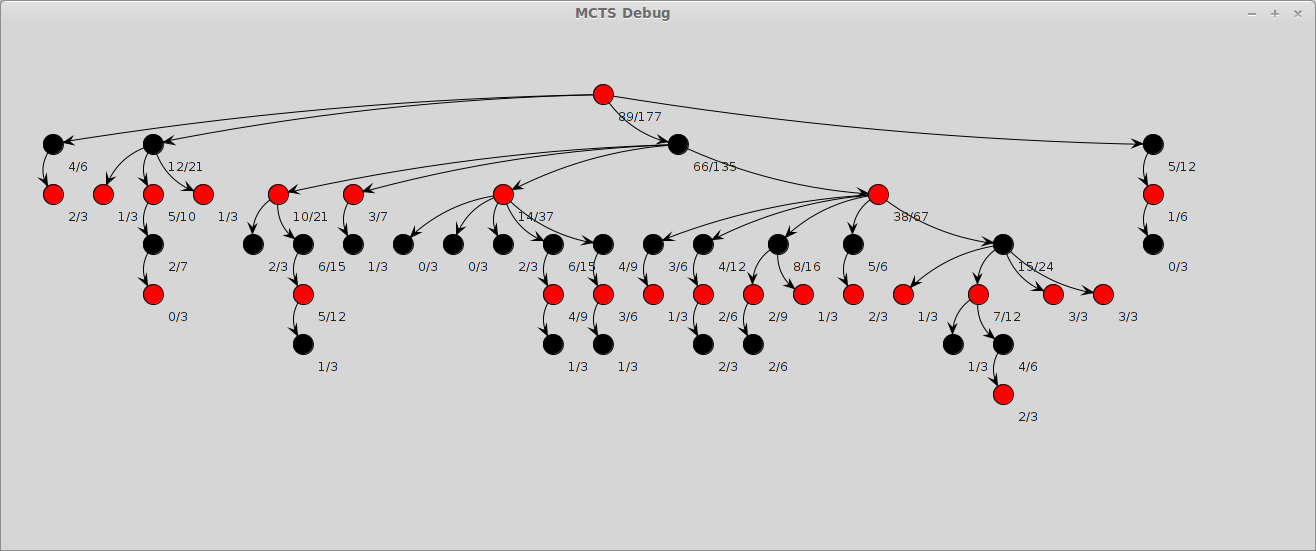
\includegraphics[width=\textwidth]{../images/mcts_tree}
                \label{fig:gull}
        \end{subfigure}
        \vspace{-20pt}\caption{The Monte Carlo Game Tree as visualized using JUNG whilst playing chess. The colors correspond to the two different players.}\label{fig:2}
\end{figure*}

Our full implementation can be found at the following GIT repository.
\begin{framed}
\scriptsize
https://github.com/samuelaustin/RandomizedAlgorithms\_Lab2
\end{framed}
\normalsize
It can be cloned with the following command.
\begin{framed}
\scriptsize
git clone git\@github.com:samuelaustin/RandomizedAlgorithms\_Lab2.git
\end{framed}
\normalsize
Our implementation is in the folder gpp-base/src/user/.

\section{Methods}
Testing the performance of a MCTS algorithm is hard due to the randomized aspects of the algorithm and the time required for playing out whole games. For the same game the algorithm can return different moves based on the paths in the tree it explored. The only way of estimating the effectiveness of the algorithm is by playing against other AI’s or human players and seeing how often it wins.

To test the effectiveness of our implementation we ran a number of games of ‘Small Checkers’ against the SampleMonteCarloGamer included in the GGP framework. This player is a pure Monte Carlo implementation which does not build a tree from its search results. As our implementation retains information from previous search iterations we expect it to perform better than the SampleMonteCarloGamer.

While playing, for each move every player gets a certain amount of time in which to perform calculations to decide its move. In our tests we gave the players 15 seconds to perform a move.

\section{Analysis and Results}
Due to time constraints we were not able to complete a large number of games. We managed to complete ten games, of which each game was won by our implementation. Three of the ten games were decided after 101 moves based on the remaining pieces left on the board. Based on this we can claim that our implementation performs better than the pure Monte Carlo approach. However, to be more certain we would have to play a larger number of games. The files containing the games can be found in the github repository under ggp-saved-games/.

It would be interesting to play against other MCTS based players to see how our implementation compares to similar ones.

\section{Conclusion}
The monte carlo game tree search algorithm is a powerful algorithm and lies at the heart of todays most advanced artificial intelligence systems. The algorithm performs well given enough computational resources and time. We were successful in implementing the algorithm producing a marginally good checkers player. The amount of computation time given for each move has a large affect on how well the algorithm performs.

An advantage of the MCTS approach is that its behaviour is hard to predict. This means it is difficult to create a player that exploits the weaknesses of the MCTS implementation. This is direct benefit gained from the randomized parts of the algorithm. Additionally, the algorithm is able to sample a fairly large portions of the search space in a small amount of time. This means the algorithm finds relatively good moves fairly quickly, making it a potentially potent opponent for human and AI players alike.

Our implementation could be improved by considering game specific heuristics to guide the searching through the tree. However, for this assignment we were mainly interested in the performance of a pure MCTS implementation.

\bibliographystyle{plain}
\bibliography{mybib} 
\end{document}
